\begin{frame}
    \frametitle{Body biasing injection: LIRMM BBI platform}
    \begin{columns}

        \begin{column}{0.2\textwidth}
            \centering
            \begin{figure}
                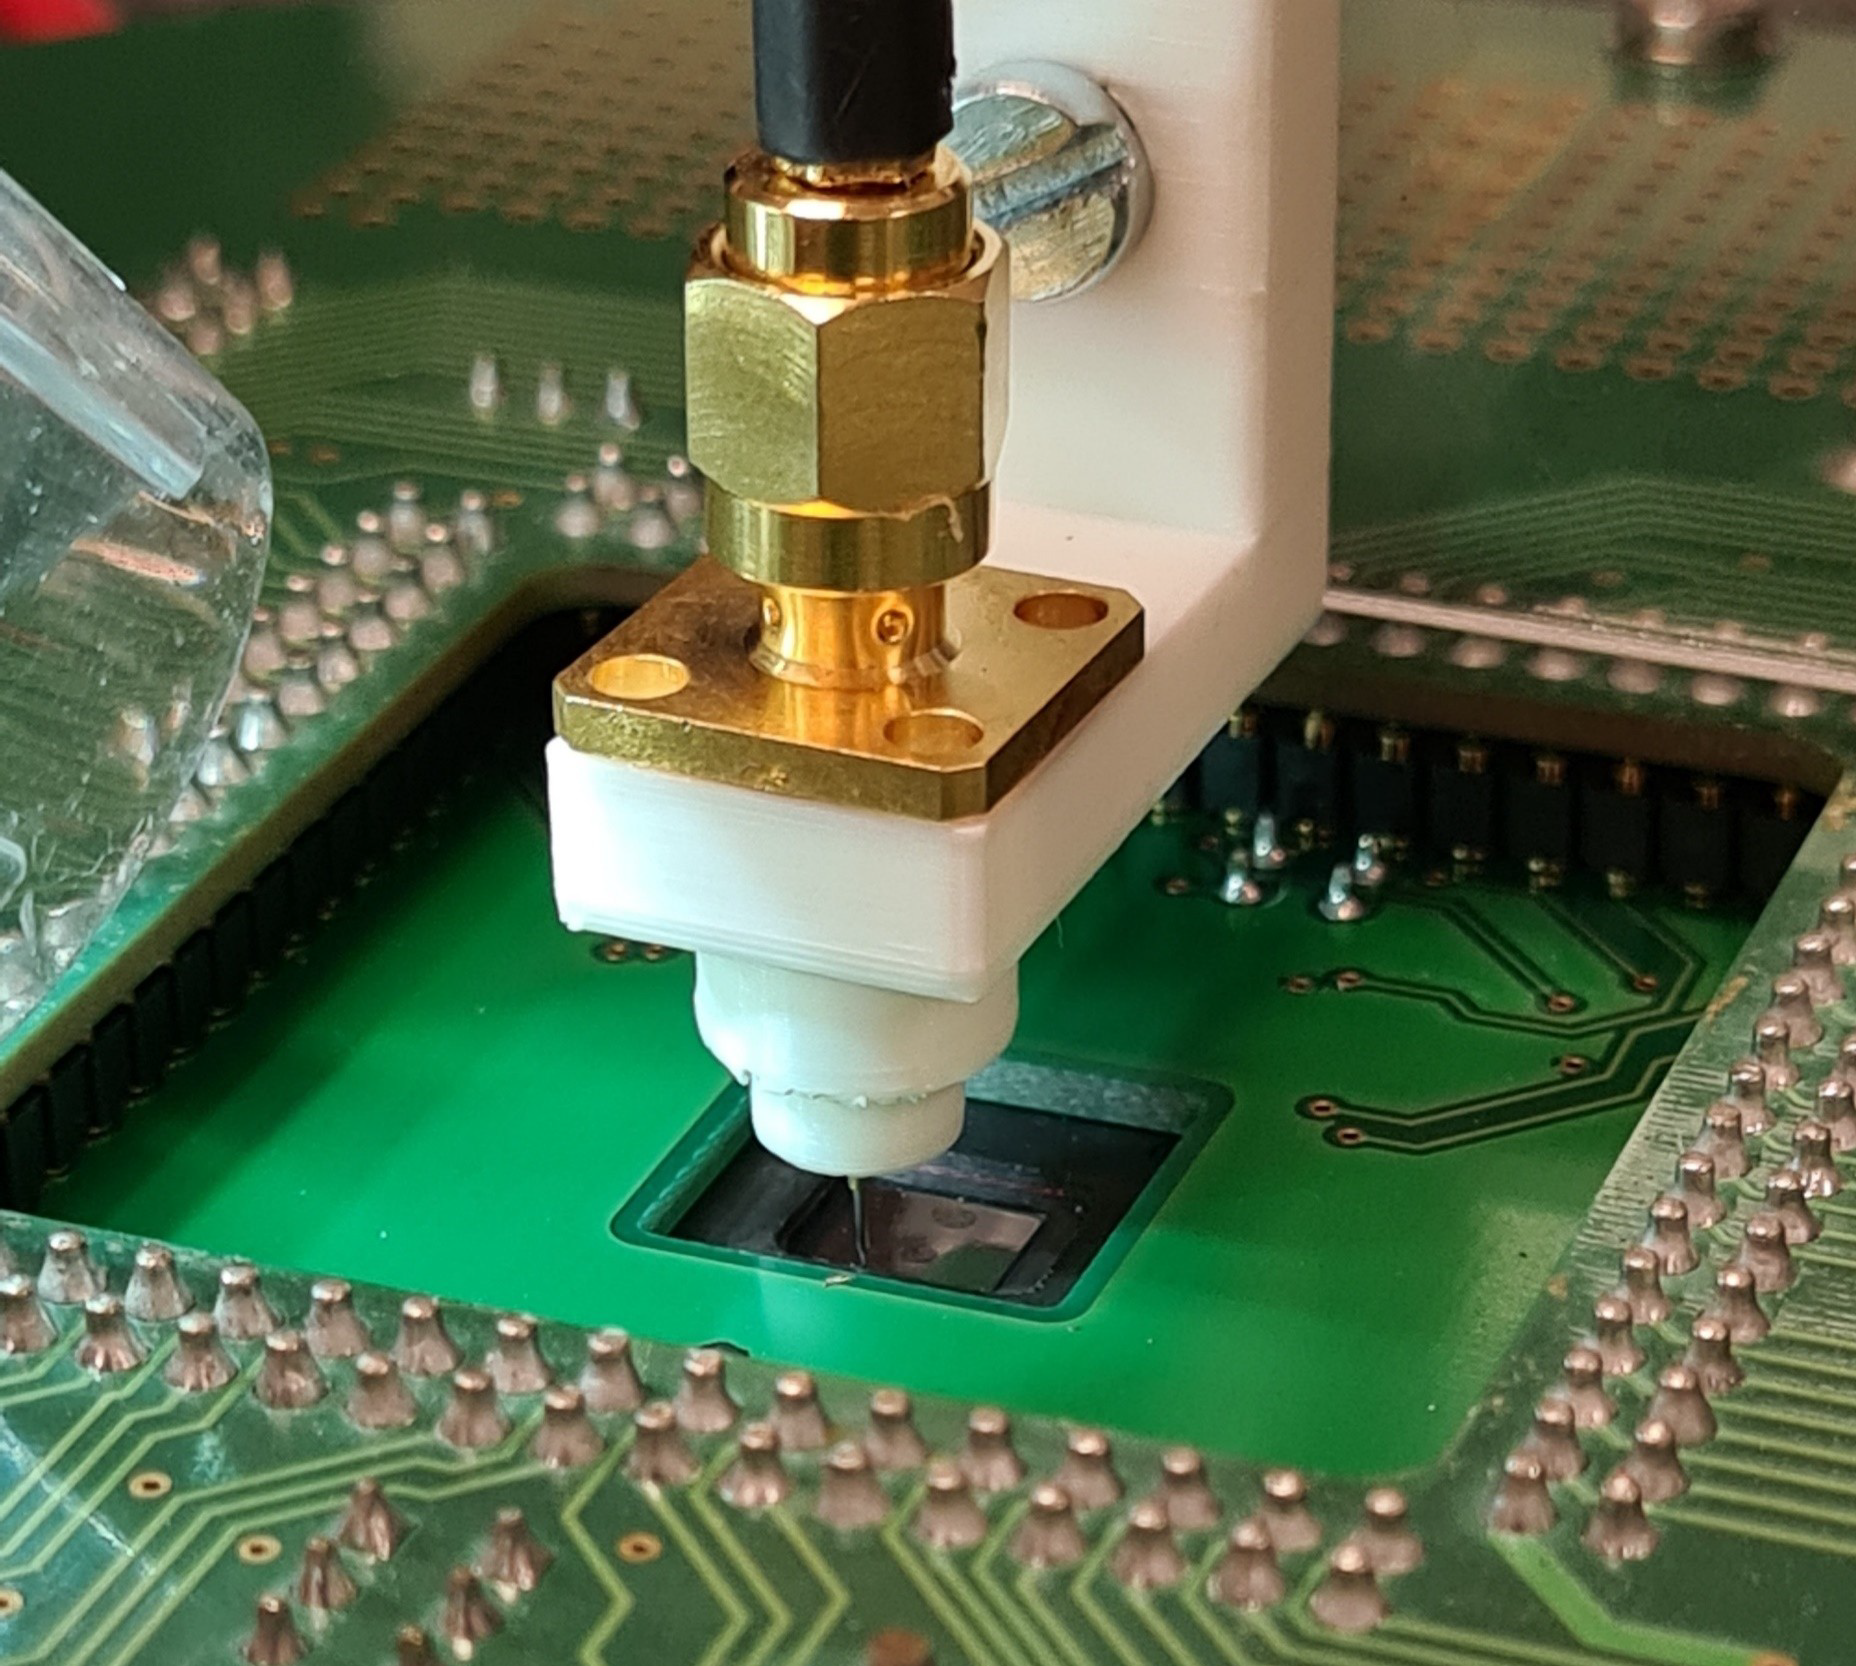
\includegraphics[width=\textwidth]{sondeBBI_loin_raw.png}
            \end{figure}
            \begin{figure}
                \includegraphics[width=\textwidth]{pointeBBI2.png}
            \end{figure}
        \end{column}

        \barsep

        \begin{column}{0.8\textwidth}
            \centering
            \begin{figure}
                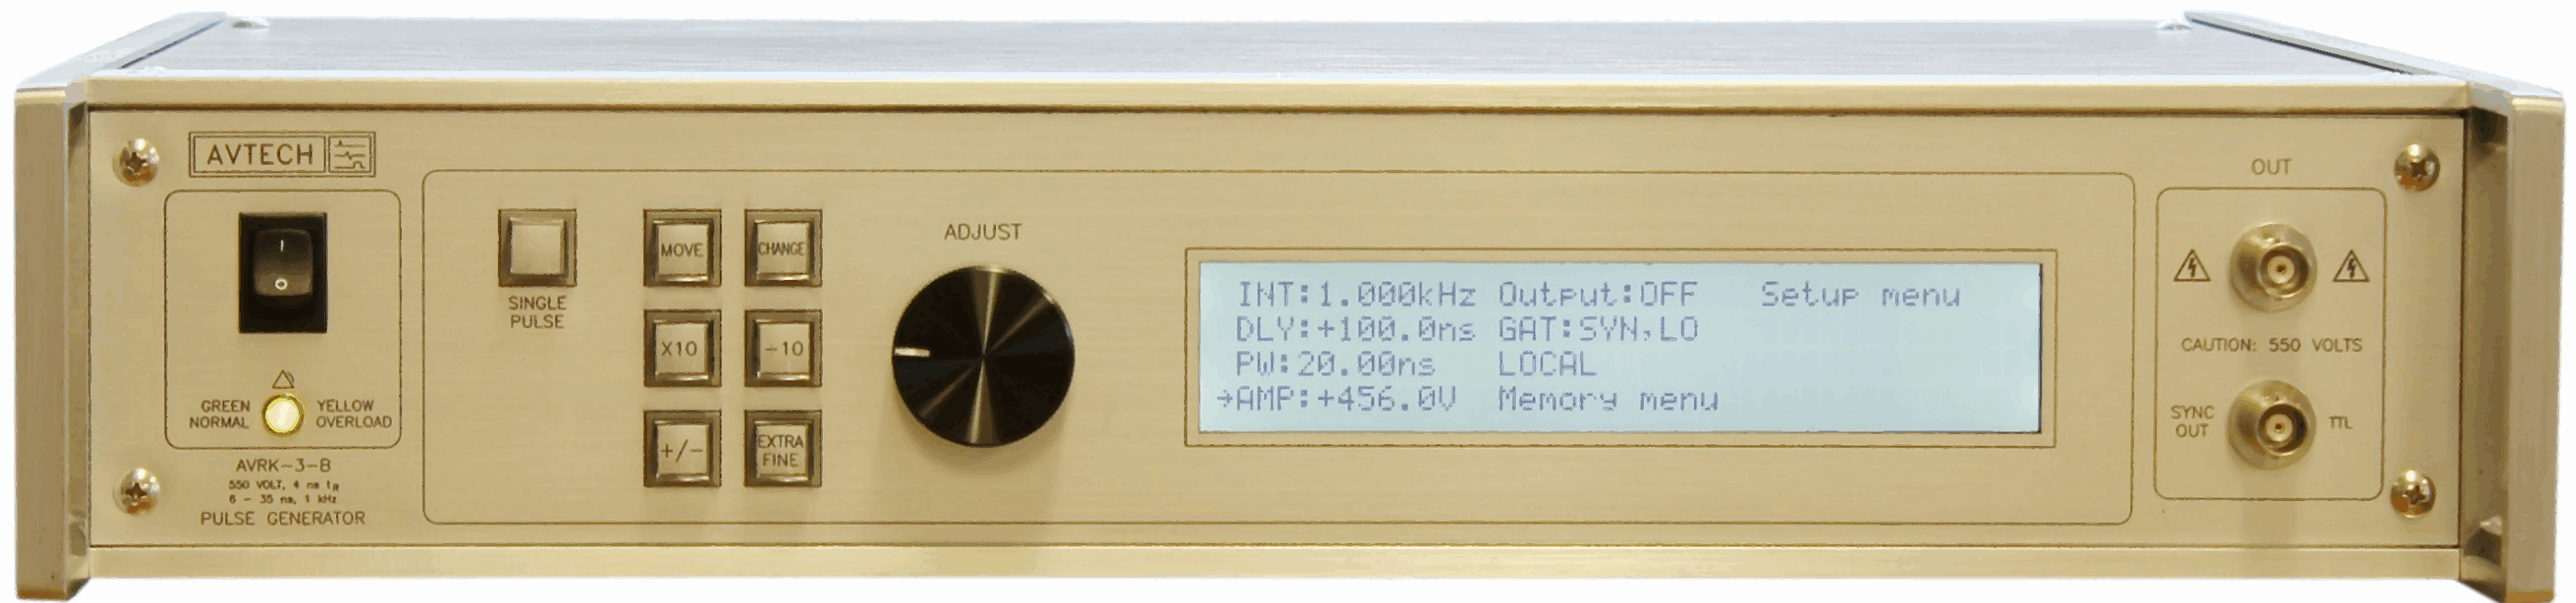
\includegraphics[width=0.6\textwidth]{avrk4b.pdf}
            \end{figure}
            \begin{itemize}
                \item Custom BBI probe;
                \begin{itemize}
                    \item Spring-loaded metal probe;
                    \item Custom 3D printed housing;
                    \item SMA connector;
                \end{itemize}
                \item AVTECH AVRK-4-B high voltage pulse generator.
                \item \textcolor{red}{Ajouter caractéristiques plateforme}
            \end{itemize}
        \end{column}

    \end{columns}
\end{frame}

\begin{frame}
    \frametitle{Body Biasing Injection: thesis objectives}
    \begin{itemize}
        \setlength\itemsep{1em}
        \item What is the spatial resolution of BBI?
        \item What is the time resolution of BBI?
        \item Is thinning the substrate useful in any way?
        \item How faults occur in a BBI context?
        \item How to model BBI?
    \end{itemize}
\end{frame}

\begin{frame}
    \frametitle{Thesis agenda}
    \begin{itemize}
        \setlength\itemsep{1em}
        \item Body Biasing Injection platform enhancements;
        \item Integrated circuits modeling for BBI;
        \item Enhanced simulation flow;
        \item Substrate thinning analysis in a BBI context.
        \item Conclusion and perspectives
    \end{itemize}
\end{frame}
